\documentclass[letterpaper]{article}
\usepackage{amsmath}
\usepackage{array}
\usepackage{color}
\usepackage{graphicx}
\usepackage{float} % utiliser H pour forcer a mettre l'image ou on veut
\usepackage{lscape} % utilisation du mode paysage
\usepackage{mathbbol} % permet d'avoir le vrai symbol pour les reels grace a mathbb
\usepackage{enumerate} % permet d'utiliser enumerate
\usepackage{moreverb} % permet d'utiliser verbatimtab : conservation la tabulation
\usepackage{stmaryrd} % permet d'utiliser \llbrackedt et \rrbracket : double crochet
\usepackage[noabbrev]{cleveref} % permet d'utiliser cref and Cref
\usepackage{caption} % permet d'utiliser subcaption
\usepackage{subcaption} % permet d'utiliser subfigure, subtable, etc
\usepackage[margin=1.in]{geometry}

\newcommand\bn{\boldsymbol{\nabla}}
\newcommand\bo{\boldsymbol{\Omega}}
\newcommand\br{\mathbf{r}}
\newcommand\la{\left\langle}
\newcommand\ra{\right\rangle}
\newcommand\bs{\boldsymbol}
\newcommand\red{\textcolor{red}}
\newcommand\blue{\textcolor{blue}}
\newcommand\ldb{\{\!\!\{}
\newcommand\rdb{\}\!\!\}}
\newcommand\llb{\llbracket}
\newcommand\rrb{\rrbracket}
\newcommand\mc{\mathcal}

\renewcommand{\(}{\left(}
\renewcommand{\)}{\right)}
\renewcommand{\[}{\left[}
\renewcommand{\]}{\right]}

\usepackage{setspace}
%\doublespacing

\begin{document}
%\title{Discontinuous Finite Element Solution for Diffusion Equations on Arbitrary Polygonal Meshes}
\title{Discontinuous Finite Element Solution of the Diffusion Equation on Arbitrary Polygonal Meshes}
\author{} 
\date{}
\maketitle

%%%%%%%%%%%%%%%%%%%%%%%%%%%%%%%%%%%%%%%%%%%%%%%%%%%%%%%%%%%%%%%%%%%%%%%%%%%%%%%%%%%%%%%%
\section{Introduction} \label{sec_intro}
%%%%%%%%%%%%%%%%%%%%%%%%%%%%%%%%%%%%%%%%%%%%%%%%%%%%%%%%%%%%%%%%%%%%%%%%%%%%%%%%%%%%%%%%

This paper deals with a discontinuous finite elemt spatial discretizations of the radiation 
diffusion equation on arbitrary polygonal grids, with and without adaptive mesh refinement. 
Radiation diffusion is an asymptotic limit of the radiation transport equation and can be 
written in the following form:
\begin{equation} \label{eq:radiation_diffusion}
- \div  D(\vr) \grad E(\vr) + \sigma_a(\vr) E(\vr) = Q(\vr) ,
\end{equation}
where $E$ is the radiation energy intensity, $D$ is a diffusion coefficient, $\sigma_a$ is 
an opacity coefficient, and $Q$ is the source.

Several spatial discretizations have been proposed to solve \eqt{eq:radiation_diffusion} on
arbitrary polygons (2D) and polyhedra (3D) \cite{Wachspress,PalmerLLNL,Palmer2005,MorelHall,MorelShashkov,%
BaileyAdams2008,KutnetsovMimetic}. 

Wachspress \cite{Wachspress} developed a family of rational polynomial functions that can be employed
as basis functions in a finite element method on polygonal/polyhedral grids. This yields
symmetric positive-definite (SPD) matrices but (i) the finite element integrals must be carried out 
numerically and (ii) the Jacobian of the transformation becomes zero on degenerate cells 
(such as the ones shown on \fig{fig:amr_schematics}). Palmer \cite{PalmerLLNL,Palmer2005}
proposed a node-based finite volume method that enforces particle balance over dual cells,
where a dual cell is defined as the union of all corners surrounding a given vertex $p$ and where  
a corner is a quadrilateral defined by vertex $p$, the cell center, and the midpoint
of the edges that contain vertex $p$. On a triangular grid, Palmer's scheme is equivalent 
to linear continuous finite elements with ``mass-matrix lumping''. The method is 
second-order accurate but the discretization of the diffusion equation using Palmer's method 
does not result in SPD matrices.







In this paper, we are interested in solving the diffusion equation on a
polygonal mesh. First, we want to point the usefulness of using polygonal
cells to discretize the domain of a problem. Such cell type presents a big 
advantage over traditional cells type (triangles and rectangles): polygonal 
cells allow for meshing flexibility. Boundary layer meshes can easily be set 
up, polygonal meshes can be generated from triangular meshes, and polygons 
can be included locally in existing meshes to improve mesh quality. Existing 
meshing tools such as MSTK \cite{mstk} and the Computational Geometry Algorithms 
Library \cite{cgal} may be employed to process polygonal meshes. For 
instance, the radiation transport code PDT and the CFD codes Fluent and OpenFoam 
offer polygonal mesh and solver capabilities. The following features of polygonal
cells are noteworthy:
\begin{description}
  \item[Optimal partition of the space minimizing boundary/interior ratio]
  \item[Reduced number of unknowns:] To illustrate this, we assume
    one unknown per vertex in every cell, which is standard for linear discontinuous
    finite element transport discretizations that perform well in the thick
    diffusive regime. In the 2D hexagonal example of \Cref{fig_hex_vs_tri},
    the number of unknowns would be six (one unknown per vertex). Using
    triangular cells, the same hexagon would have to be split into four
    triangles at least (thus 12 unknowns) or possibly six triangles to
    preserve symmetry (thus 18 unknowns in that case). Similarly, using
    quadrilateral cells, the hexagon would be bisected into two quadrilaterals
    at least (8 unknowns), but divisions into three of four quadrilaterals are
    also possible (thus, 12 or 16 unknowns).
    \begin{figure}[H]
      \centering
      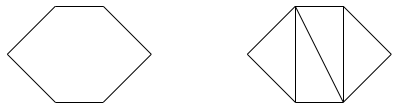
\includegraphics[width=5cm]{hex_tri_cells}
      \caption{Hexagonal cell versus triangle cells}
      \label{fig_hex_vs_tri}
    \end{figure}
  \item[Transition elements and Adaptive Mesh Refinement:] Solvers based on
    arbitrary polyhedral cells can easily handle cells with various number of
    edges. This can be particularly useful for simulations
    with Adaptive Mesh Refinement (AMR) \cite{Jessee1998,Baker2002,Wang2010a}, 
    without having to deal with the implementation of data structures to handle 
    hanging nodes \cite{Solin2008,Bangerth2007,Arnold2000}. On \Cref{fig_amr_cells}, 
    the left cell is a pentagon whereas the two cells on the right are 
    quadrilaterals. A method based on a piecewise linear discretization can
    handle locally adapted meshes without any special treatment or further
    approximation of the coupling between cells.
    \begin{figure}[H]
      \centering
      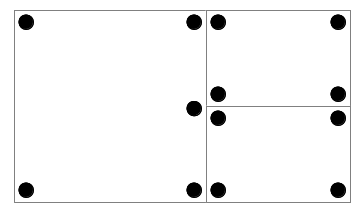
\includegraphics[width=5cm]{amr}
      \caption{AMR mesh}
      \label{fig_amr_cells}
    \end{figure}
\end{description}
Several discretization methods have been developed for arbitrary polygonal
meshes: Palmer's method \cite{Palmer2001}, mimetic finite differences
\cite{Lipnikov2004,Hyman2002,Kuznetsov2004,Brezzi2005},
Wachspress' rationale finite element \cite{Wachspress1975},
CFEM-based DFEM \cite{Warsa2008}, PWLC \cite{Bailey2008a}, PWLD 
\cite{Stone2003,Bailey2008,Bailey2008a}, and PWBLD \cite{Bailey2011}. In this
research, we focus on using PWLD to discretize the diffusion equation. The
PWLD discretization employs discontinuous finite elements and has been used to
discretize the transport equation. Using it to discretize the diffusion
equation is an important step in order to create a Diffusion Synthetic
Acceleration scheme \cite{Adams2002,Wang2010}.
In \Cref{sec_review}, we review different discretizations that can be used on
polygonal cells to discretize the diffusion equation. In \Cref{sec_ip}, we
use the PWLD finite elements to discretize the diffusion
equation. In \Cref{sec_amr}, we introduce the Adaptive Mesh Refinement
technique (AMR). In \Cref{sec_results}, we show some numerical results. We finish
in \Cref{sec_conc} by giving our conclusions.

\section{Review of discretizations for polygonal meshes} \label{sec_review}
In this Section, we review different discretizations that can be used on polygonal
meshes at the exception of the PWLD discretization which will be introduce in
the next Section.
\subsection{Palmer's method}
Palmer's method is a node- or point-based method \cite{Palmer2001}. This
discretization is second order and uses a finite volume approach: the
particle balance is enforced by integrating over a control volume. The control 
volume is the union of all corners surrounding a vertex $p$. A corner is a
quadrilateral defined by the vertex $p$, the cell-center $c$, and the midpoint
of the edges $e$ that contain the point $p$. On a triangular grid, the
scheme is equivalent to linear continuous finite elements with ``mass-matrix
lumping''. This method works for any polygonal cell even concave polygon. The
main disadvantage of Palmer's method is that the discretization of the
diffusion equation does not lead to symmetric system in the general case.
\subsection{Mimetic finite differences}
Mimetic methods, such as mimetic finite differences (MFD), mimic properties of
mathematical and physical models, such as: tensor and vector calculus,
conservation laws, symmetry preservation, solution positivity and
monotonicity, and asymptotic limits (e.g., diffusion limit), on polygonal and
polyhedral meshes. The most important part of MFD is the definition of a scalar
product which satisfies stability and consistency some conditions
\cite{Brezzi2005}. However, this scalar product is not unique and therefore,
multiple MFD methods exists. MFD is efficient even on concave polygons
\cite{Kuznetsov2004}. MFD methods are related to mixed finite elements.

%\red{An important (mimetic) property of operators div and $K\bn$ is expressed
%  by integration by part formula:
%  \begin{equation}
%    \int_{\bo} K^{-1}\bs{u} \cdot (K\bn p)dV = - \int_{\bo} (div\ \bs{u}) p\ dV
%  \end{equation}
%  which holds for any $p \in H_0^1(\bo)$ and $\bs{u}\in H_{div}(\bo)$.\\
%  The MFD method mimics this property by replacing integrals and operators by
%  their discrete counterparts:
%  \begin{equation}
%    [\bs{U},GRAD\ P]_X = -[DIV\ \bs{U},P]_Q
%  \end{equation}
%which holds for any vectors of degrees of freedom $P$ and $\bs{U}$. MFD
%connected to mixed finite elements. Works with mixed cells.}
%\red{Mimetic numerical methods mimic crucial properties of mathematical and
%  physical models on arbitrary on polygonal and polyhedral meshes:
%  \begin{itemize}
%    \item tensor and vector calculus
%    \item conservation laws
%    \item symmetry preservation
%    \item solution positivity and monotonicity
%    \item asymptotic limits (e.g., diffusion limit in radiation transport
%      models)
%  \end{itemize}}
%\red{\cite{Lipnikov2004} only quadrilaterals with at most one hanging node per edge. 
%  SO can be applied to many forms of the diffusion equation, but here we consider
%the first-order form of the diffusion equation. Use local SO.
%\begin{itemize}
%  \item there are two different support-operators methods, they both
%        give the same cell-center intensity solutions:
%    \begin{itemize}
%      \item one has intensity unknowns located only at cell centers: the
%        diffusion matrix is dense.
%      \item one has intensity unknowns located at both cell centers and face
%        centers: the diffusion matrix is space. The cell-center unknowns are
%        locally eliminated, resulting in a reduced system consisting only of
%        the face-center unknowns. The method is called the local SO method.
%    \end{itemize}
%  \item local SO is composed of two steps:
%    \begin{itemize}
%      \item consider each cell in the domain as a independent domain and
%        generate an independent discretization for each cell (identical to
%        what is done for standard quadrilateral meshes)
%      \item obtain a global discretization by imposing continuity of the
%        intensity and continuity of the normal component of the flux across
%        cell interfaces. 
%    \end{itemize}
%\end{itemize}
%\cite{Hyman2002} the mimetic FDM are based on discrete of first-order
%coordinate-invariant operators, it is natural to write the diffusion equation
%as a system of first order equations.
%\cite{Kuznetsov2004} works for any polygons. Used in geophysics $->$ the equation is
%split in two first-order equations.
%\begin{itemize}
%  \item exact for linear solution
%  \item SPD
%\end{itemize}
%\cite{Brezzi2005} the key element of the MFD method is the scalar product in the
%space of discrete velocities which should satisfy the stability assumption and
%the consistency assumption. It turns out that such a scalar product is not
%unique.
%\begin{enumerate}
%  \item specify the degrees of freedom for the primary variables
%  \item define suitable scalar products in the discrete spaces
%  \item discretize the divergence operator
%  \item define the discrete flux operator
%\end{enumerate}}
\subsection{Wachspress' rationale finite element}
Before introducing the Wachspress' basis function on a quadrilateral cell, 
we define $P_{1,2}(x,y)$ the polynomial defined by the points $(x_1,y_1)$ and
$(x_2,y_2)$:
\begin{equation}
  P_{1,2}(x,y) = (y-y_1) (x_2-x_1)-(x-x_1)(y_2-y_1).
\end{equation}  
Therefore, Wachspress' basis functions are given by:
\begin{align}
  &b_0(x,y) = k_0 P_{2,3}(x,y)P_{1,2}(x,y)/P_{4,5}(x,y),\\
  &b_1(x,y) = k_1 P_{0,3}(x,y)P_{2,3}(x,y)/P_{4,5}(x,y),\\
  &b_2(x,y) = k_2 P_{0,1}(x,y)P_{3,0}(x,y)/P_{4,5}(x,y),\\
  &b_3(x,y) = k_3 P_{1,2}(x,y)P_{0,1}(x,y)/P_{4,5}(x,y),
\end{align}
where $k_i$ are chose such that $b_i(x_i,y_i)=1$. $(x_4,y_4)$ and $(x_5,y_5)$
are the intersections of the prolongations of the edges 
of the quadrilaterals (see \Cref{fig_quadrilateral}).
\begin{figure}[H]
  \centering
  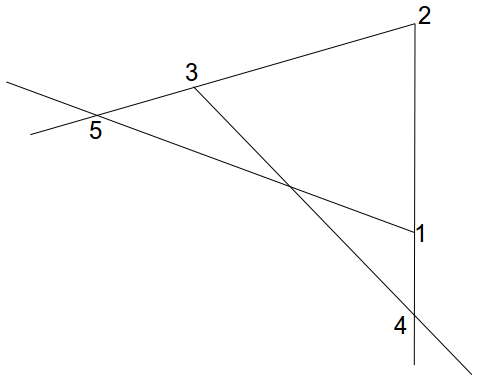
\includegraphics[width=5cm]{quadrilateral}
  \caption{Quadrilateral cell}
  \label{fig_quadrilateral}
\end{figure}
These two points uniquely defines a linear polynomial. It should be noted that 
the line defined by $(x_4,y_4)$ and $(x_5,y_5)$ does not pass through the 
quadrilateral and thus, the denominator cannot vanish (this is 
only true for convex quadrilateral). When the quadrilateral tends to a 
parallelogram, the points defining $P_{4,5}$ are moved to infinity and 
$P_{4,5}(x,y)$ tends to a constant inside the quadrilateral. By definition, 
this constant is chosen to be one for a parallelogram. For a trapezoid,
$P_{4,5}(x,y)=0$ is the equation of the line parallel to the two parallel
edges of the trapezoid which contains the intersection of the prolongations of
the two non-parallel edges. For arbitrary polygons, a non-trivial 
generalization is necessary \cite{Wachspress1975}.
%\red{\cite{Bailey2008a} he disadvantage is that the basis function integrals must
%be done numerically.
%\red{\cite{Wachspress1975} $(r;q)_2|_3$ is the value at point 3 of a quadratic
%  function containing points $r$ and $q$. This value depends on supplementary
%  data which defines the quadratic function $(r;q)_2$. Similarly
%  $[(1;2)_2(3;4)/(1;5)]|_8$ is the value of the indicated rational function
%  at point 8. For quadrilaterals: we look for a function like:
%  \begin{equation}
%    w_1(x,y) = \frac{Q_1}{(2;3)(3;4)}|_1 \frac{(2;3)(3;4)}{Q_1}
%  \end{equation}
%  We therefore seek a linear from $Q_1$ such that:
%  \begin{itemize}
%    \item $Q_1\neq 0$ within the quadrilateral
%    \item $\frac{(2;3)(3;4}{Q_1}$ is linear on both $(4;1)$ and $(1;2)$
%  \end{itemize}
%  The first property has far-reaching consequences: we must broaden our vision
%  and look outside the quadrilateral. We observe that all the linear forms
%  appearing in the triangle and parallelogram wedges were determined by the
%  sides of these figures. We shall soon see that the quadrilateral itself
%  reaches out to give us the desired linear form. First, we need the following
%  lemma: \emph{If three lines intersect at a point then the ratio of linear
%  forms which vanish on any two of these lines is constant on the third line.}
%  We choose $Q_1$ so that $(2;3)/Q_1$ is constant on side $(4;1)$ and so that
%  $(3;4)/Q_1$ is constant on side $(4;1)$ and so that $(3;4)/Q_1$ is constant
%  on side $(1;2)$. By the lemma, the first requirement is met if lines
%  $(2;3)$, $(4;1)$, and $Q_1$ have a common point of intersection and the
%  second requirement is met if lines $(3;4)$, $(1;2)$, and $Q_1$ have a common
%  point of intersection. If we define point 5 as the intersection point of
%  lines $(2;3)$ and $(1;4)$ and point 6 as the intersection of $(1;2)$ and
%  $(3;4)$, we find that $Q_1(x,y) = (5;6)$ is the unique line which meets both
%  requirements. For any convex quadrilateral, line $Q_1$ has no point in the
%  quadrilateral. Consistent candidates for all four wedges are:
%  \begin{subequations}
%    \begin{align}
%      &W_1(x,y) = k_1 (2;3)(3;4)/Q_1(x,y)\\
%      &W_2(x,y) = k_2 (3;4)(4;1)/Q_1(x,y)\\
%      &W_3(x,y) = k_3 (4;1)(1;2)/Q_1(x,y)\\
%      &W_4(x,y) = k_4 (1;2)(2;3)/Q_1(x,y)
%    \end{align}
%  \end{subequations}
%  The $k_i$ are chose so that $W_i(x_i,y_i)=1$. As the quadrilateral is
%  deformed into a parallelogram, the exterior diagonal moves to infinity and
%  the associated linear from moves to infinity and the associated linear form
%  becomes more nearly constant within the quadrilateral. We therefore let
%  $Q_1(x,y)=1$ for a parallelogram. For a trapezoid, the exterior diagonal is
%  parallel to the parallel sides and passes through the intersection point of
%  the others two sides. We note that the exterior diagonal is uniquely defined
%  as the lined that intersects the sides of the quadrilateral at all the
%  exterior intersection points of these sides and at no other points.
%A non-trivial generalization is necessary for polygons.} 
\subsection{CFEM-based DFEM}
CFEM-based DFEM stands for Continuous Finite Elements-based Discontinuous
Finite Elements. This method is very similar to the PieceWise Linear
Discontinuous finite elements (PWLD) discretization (see \Cref{subsec_pwld}). 
The scheme is second order \cite{Warsa2008}. The discretization is done by
first dividing the cells into triangles that we call sub-cells. The sub-cells
are formed by filling the polygons with triangles without adding point (type
0) or by adding the centers of the cells as the vertices of the sub-cells
(type 1). Linear DFEM are built on the triangles. Type 1 CFEM-based DFEM is
similar to PWLD but whereas PWLD eliminates the center unknown by setting it
to be the weighted average of the values at the vertexes, CFEM-based DFEM keeps 
the additional degree of freedom as an unknown. The mass matrix 
$\bs{M}$ for a given cell composed of $N$ sub-cells is assembled by looping
over the sub-cell and for each sub-cell $n$:
\begin{equation}
  \bs{M}_{t_n(u),t_n(v)} = \bs{M}_{t_n(u),t_n(v)} + \bs{M}_{n,u,v}, 
  \textrm{ for }u=1,2,3,\ v=1,2,3
  \label{mass_cfem}
\end{equation}
where $\bs{M}_n$ is the mass matrix of the $n^{th}$ sub-cell and $t_n$ is an 
indexing function which maps the index of the vertices of the sub-cells to the 
index of the vertices in the cell. The streaming matrix is given by a similar 
equation:
\begin{equation}
  \bs{L}_{t_n(u),t_n(v)} = \bs{L}_{t_n(u),t_n(v)} + \bs{L}_{n,u,v}, 
  \textrm{ for }u=1,2,3,\ v=1,2,3
  \label{stream_cfem}
\end{equation}
and the mass matrix on the edge $k$, $\bs{N}_{i,j}^{(k)} = \bs{n}_k
\int_{\partial E_k} b_i(\br) b_j(\br) d\br$, is given by:
\begin{equation}
  \bs{N}_{t_n(u),t_n(v)}^{(f_n(l))} = \left\{
    \begin{aligned}
      & \bs{N}_{n,u,v}^{(l)}, & \textrm{ if }f_n(l)\neq 0\\
      & 0, & \textrm{ otherwise }
    \end{aligned}
  \right.
  \textrm{ for } l=1,2,3,u=1,2,3,v=1,2,3
\end{equation}
where $f_n(l)$ is an indexing function to map face $l$ of the sub-cell $n$,
for $n=1,\hdots,N,$ to the corresponding face of the polygon.
\subsection{PWLC}
PWLC stands for PieceWise Linear Continuous finite elements. It is a second
order method which when used to discretize the diffusion equation produces 
a Symmetric Positive-Definite (SPD) matrix \cite{Bailey2008}. The PWL basis 
function associated to $j^{th}$ vertex is given by:
\begin{equation}
  b_j(\br) = t_j(\br) + \alpha_{c,j} t_c(\br)
\end{equation}
where the $t_j$ function is the standard linear functions defined on the
triangle formed by the $j-1^{th}$, $j^{th}$, and $j+1^{th}$ vertices:
$t_j$ equals 1 at the $j^{th}$ vertex of the cell and
0 at the $j-1^{th}$ and $j+1^{th}$ vertices. $t_c$ is
is equal to one at point $c=(x_c,y_c)$ and 0 at all the vertices, with $x_c =
\sum_{i=0}^{N_V} \alpha_{c,i} x_i$, $y_c = \sum_{i=0}^{N_V} \alpha_{c,i} y_i$,
and $\sum_{i=0}^{N_V} \alpha_{c,i} = 1$. The assembling of the mass and 
streaming matrices is similar than the one of CFEM-based DFEM. The matrices
associated to a given cell is assembled by looping over triangular sub-cells
(see \Cref{subsec_pwld}).
\subsection{PWLD} \label{subsec_pwld}
PWLD uses similar basis functions than PWLC but they are defined only on a
element. Like pointed out previously, PWLD is closely related to type 1
CFEM-based DFEM. Both methods use sub-cells to build the mass matrix and the
streaming matrix. However since for PWLD, the center unknown is eliminated,
\cref{mass_cfem,stream_cfem} become:
\begin{align}
  \bs{M}_{t_n(u),t_n(v)} &= \bs{M}_{t_n(u),t_n(v)} + w_{n,u,v}\bs{M}_{n,u,v}, 
  \bs{L}_{t_n(u),t_n(v)} &= \bs{L}_{t_n(u),t_n(v)} + w_{n,u,v} \bs{L}_{n,u,v}, 
\end{align}
for $u=1,2,3,\ v=1,2,3$. $w_{n,u,v}$ is a weighting function which is used to
eliminate the extra unknown. The value of $w_{n,u,v}$ depends on
$\alpha_{c,j}$.
\subsection{PWBLD}
PWBLD stands for PieceWise Bi-Linear Discontinuous finite elements. This 
discretization is very similar to the PWLD discretization. When using PWBLD, 
the convex polygonal cell is divided on quadrilateral sub-cells instead of
triangular sub-cells for PWLD \cite{Bailey2011}. On these quadrilaterals, 
the bi-linear basis functions are used. If the cell is 
quadrilateral, PWBLD finite elements are identical to bi-linear discontinuous 
finite elements.

\section{Interior Penalty method} \label{sec_ip}
The discretization of the diffusion equation using discontinuous finite
elements is not as straightforward as it is when using continuous finite
elements. To discretize the diffusion equation with discontinuous finite elements, 
we apply the interior penalty method \cite{Kanschat2007}:
\begin{equation}
  -\bn D \bn \phi + \Sigma_a \phi = Q_0\ \textrm{ for } \br \in \mc{D},
\end{equation}
\begin{equation}
  \frac{1}{4}\phi - \frac{1}{2} D \partial_n \phi =0\ \textrm{ for } \br \in
  \partial \mc{D}^d,
\end{equation}
and
\begin{equation}
  -D \partial_n \phi = J^{inc}\ \textrm{ for } \br \in \partial \mc{D}^n,
\end{equation}
where $D$ is the diffusion coefficient, $\phi$ is the scalar flux, $\Sigma_a$
is the absorption cross section, $Q_0$ is a volumetric source, $J^{inc}$ is an
incoming current, $\mc{D}$ is the domain, $\partial \mc{D}^d$ is the boundary 
where Dirichlet conditions are applied, and $\partial \mc{D}^n$ is the boundary 
where Neumann conditions are applied.\\ 
After symmetrization, we get the SPD equation:
\begin{equation}
  a(\tilde{\phi},b) = l(b),
\end{equation}
where:
\begin{equation}
  \begin{split}
    a (\tilde{\phi},b) =& \(\Sigma_a \tilde{\phi},b\)_{\mc{D}} + 
    \(D\bn\tilde{\phi},\bn b\)_{\mc{D}} +
    (\kappa_e\ldb\tilde{\phi}\rdb,\ldb b \rdb)_{E_h^i}\\
    &+ \(\ldb\tilde{\phi}\rdb,\llb D\partial_n b \rrb\)_{E_h^i}+ \(\llb D
    \partial_n \tilde{\phi}\rrb,\ldb b \rdb\)_{E_h^i}\\
    &+ \(\kappa_e \tilde{\phi}, b\)_{\partial \mc{D}^d}
    -\frac{1}{2}\(\tilde{\phi},D\partial_n b\)_{\partial \mc{D}^d}
    -\frac{1}{2}\(D\partial_n\tilde{\phi},b\)_{\partial \mc{D}^d}
  \end{split}
\end{equation}
and: 
\begin{equation}
  l(b) = (Q_0,b)_{\mc{D}} + (J^{inc},b)_{\partial
  \mc{D}^r},
\end{equation}
with $\tilde{\phi}=(\phi_1 b_1,\hdots, \phi_N b_N)^T$, $b = (b_1,\hdots,b_N)$,
$b_i \in W_{\mc{D}}^h$ $\forall i \in (1,\hdots,N)$,
the mesh $\mc{T}_h$ is used to discretize $\mc{D}$ into nonoverlapping linear
elements $K$, such that the union of the elements fully covers $\mc{D}$. The
finite dimensional polynomial space is $W_{\mc{D}}^h = \{f \in L^2(\mc{D});
f|_K \in V_p(K), \forall K \in \mc{T}_h$\}, where $V_p(K)$ is the space of
polynomials of degree up to $p$ on element $K$; the set of interior is $E_h^i
= \cup _{K_1,K_2\in \mc{T}_h}(\partial K_1 \cap \partial K_2)$. We also
define:
\begin{align}
  \ldb \phi \rdb &= \phi^+ - \phi^-,\\
  \llb \phi \rrb &=  \frac{\phi^++\phi^-}{2},
\end{align}
with $\phi^{\pm} = \lim_{s\rightarrow 0^{\pm}} \phi(\br+s \bs{n}_e)$, where
$\bs{n}_e$ is the normal unit vector associated with an edge $e$. On the boundary, 
the normal vector has to be oriented outward whereas the orientation on an
interior edge is arbitrary.\\
The penalty parameter $\kappa_e$ is given:
\begin{equation}
  \kappa_e = \left\{
    \begin{aligned}
      &\frac{c(p^+)}{2}\frac{D^+}{h_{\bot}^+}+\frac{c(p^-)}{2}
      \frac{D^-}{h_{\bot}^-} & \textrm{ on interior edges, i.e., } e \in
      E_h^i,\\
      & c(p)\frac{D}{h_{\bot}} & \textrm{ on boundary edges, i.e., } e\in
      \partial \mc{D},
    \end{aligned}
    \right.
\end{equation}
where $c(p) =Cp(p+1)$, $C$ is a constant (we used $C=2$), $p$ is the
polynomial order,  and $h_{\bot}$ is the length of the cell in the direction 
orthogonal to edge $e$. The + and - symbols represent the values on either 
side of an edge. On triangular cells, $h_{\bot}$ is $\frac{2A}{L_e}$ where $A$
is the area of the triangle and $L_e$ is the length of the edge $e$. However
when the cells are not triangular, there is no simple simple way to compute
$h_{\bot}$. To simplify this, we assume that the polygonal cells are not too
far from being regular polygonal cells. In such cases, if the cell has an even
number of edges, the orthogonal length equals two times the apothem, i.e., two
times the segment between the midpoint of a side of the polygon and the center
of this polygon $\(\textrm{apothem}=2\times
\frac{\textrm{area}}{\textrm{perimeter}}\)$. If the cell has an odd number of
edges, the orthogonal length is given by the apothem plus the circumradius,
i.e., the radius of the circle circumscribed to the polygon
$\(\textrm{circumradius}=\sqrt{\frac{2\times\textrm{area}}{V \sin
\(\frac{2\pi}{N_V}\)}}\)$. Therefore, $h_{\bot}$ is given by
\Cref{ortho_length}.
\begin{table}[H]
  \begin{centering}
    \begin{tabular}{|c|c|c|c|c|}
      \hline
      Number of edges & 3 & 4 & $> 4$ and even & $>4$ and odd \\
      \hline
      $h_{\bot}$ & $2\times \frac{\textrm{area}}{L_e}$ &
      $\frac{\textrm{area}}{L_e}$ & $4\times
      \frac{\textrm{area}}{\textrm{perimeter}}$ &
      $2\times \frac{\textrm{area}}{\textrm{perimeter}} +
      \sqrt{\frac{2\times\textrm{area}}{V \sin\(\frac{2\pi}{N_V}\)}}$\\
      \hline
    \end{tabular}
    \caption{Orthogonal length of the cell for different cells.}
    \label{ortho_length}
  \end{centering}
\end{table}

\section{Adaptive Mesh Refinement} \label{sec_amr}
In this Section, we introduce Adaptive Mesh Refinement (AMR)
\cite{Jessee1998,Wang2010a,Ragusa2010}. The goal of AMR is to refine the mesh
where it is necessary while keeping the mesh as coarse as possible everywhere
else. It is common to have problems where the solution varies quickly on a
small part of the domain (e.g. boundary layers) where the mesh needs to be
very fined and is smooth on the rest of the domain where large cells can be
used. AMR allows to create such a mesh automatically.AMR requires an \emph{a
posteriori} error indicator to decide which cells should be refined. In this
work, the jump-based error indicator on element $K$ is given by \cite{Wang2010a}:
\begin{equation}
  \eta_K = \frac{\int_{\partial K} \ldb\phi_K\rdb^2}{\|\Phi_K\|_2^2},
  \label{error_indic}
\end{equation}  
is used. This error indicator is based on the on the jump of the scalar flux between
two cells. The larger the jump is the larger the error indicator. Given that
the solution of the diffusion equation is continuous, \cref{error_indic} is a
good error indicator. 

The way the adaptive mesh refinement is used in our code is the following:
\begin{enumerate}
  \item The solution is computed on a coarse mesh.
  \item The error indicator for each cell is computed.
  \item All the cells $K$ such that $\eta_K > \epsilon \max_{J} \eta_J$ where
    $\epsilon \in [0,1]$ are flagged for refinement.
  \item The flagged cells are refined.
  \item The solution on the coarse mesh is projected on the fine mesh.
  \item Go back to 1.
\end{enumerate}

When a discretization that does not allow polygonal cells is used, the
refinement of the mesh created hanging nodes. When the discretization allows
polygonal cells, hanging nodes are not necessary. Every time a hanging node
would be needed, one edge is added to 2 cells.

\section{Results} \label{sec_results}
In this Section, we compare the solution of the problem on an uniform mesh
with the one on Z-mesh \cite{Stone2003}. We also show that the
discretization used can easily handle unstructured polygonal grid. Finally, we
conclude this section with an example of AMR mesh.
\subsection{Z-mesh}
The Z-mesh is defined as in \Cref{fig_z_mesh} where $\alpha$ is a parameter
$\in [0,0.5]$. 
\begin{figure}[H]
  \centering
  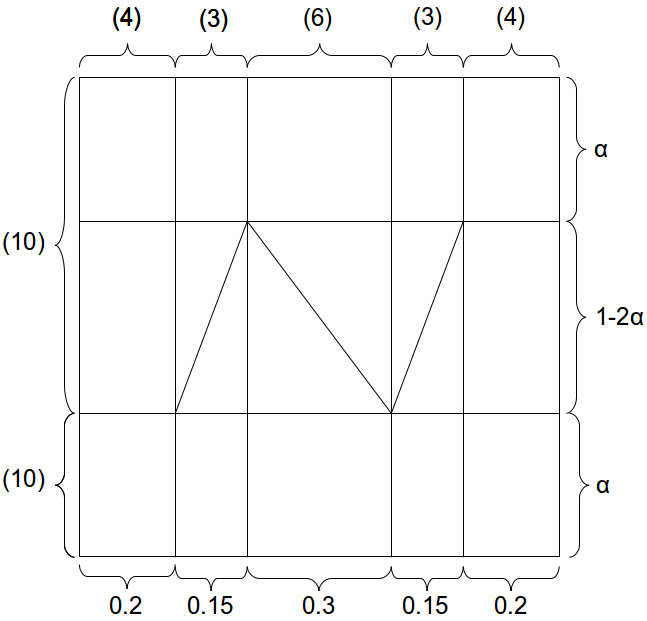
\includegraphics[width=5cm]{z_mesh}
  \caption{Z-mesh ((x) is the number of divisions and Y is the distance in cm)}
  \label{fig_z_mesh}
\end{figure}    
We compare the solution of the diffusion equation using the Z-mesh
\Cref{z_mesh_sol} with $\alpha=0.2$ with the one obtained using an uniform \Cref{u_mesh_sol}. 
The domain is 1cm by 1cm and is discretized using 20 by 20 cells. All the 
boundary conditions are vacuum. The medium is homogeneous $\Sigma_a = 0.5 cm^{-1}$ 
and $D=2$. There is a uniform source of intensity 1.                  
\begin{figure}[H]
  \centering
  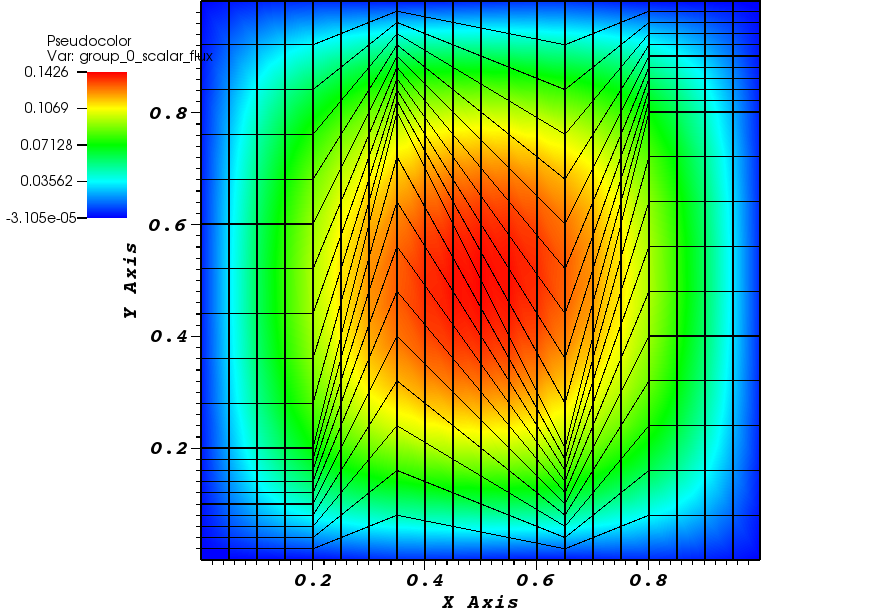
\includegraphics[width=5cm]{z_mesh_sol}
  \caption{Scalar flux on the z-mesh}
  \label{z_mesh_sol}
\end{figure}
\begin{figure}[H]
  \centering
  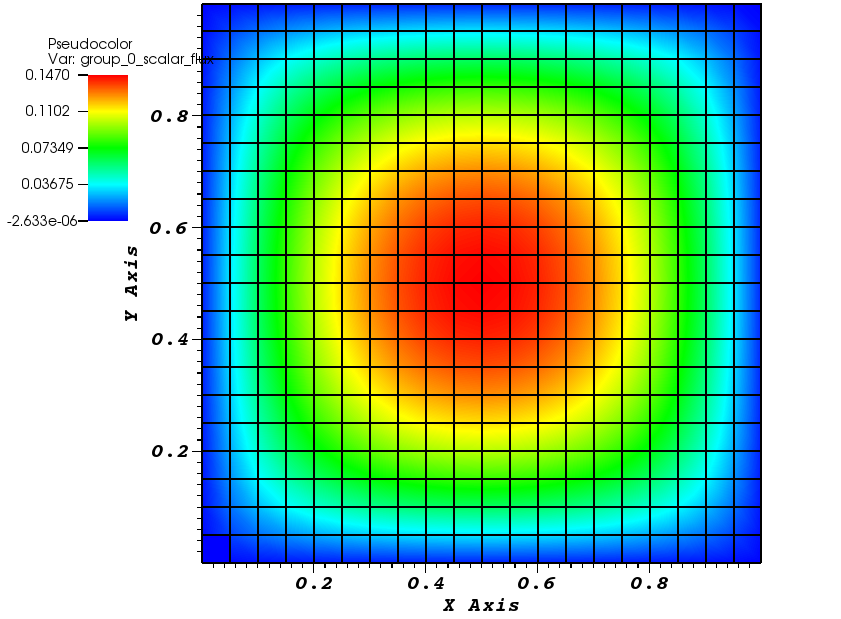
\includegraphics[width=5cm]{pwld_uniform_sol}
  \caption{Scalar flux on the uniform mesh}
  \label{u_mesh_sol}
\end{figure}
\subsection{Randomized polygonal grid}
\subsection{AMR}
The AMR problem is composed of two regions, see \Cref{amr_regions}.
\begin{figure}[H]
  \centering
  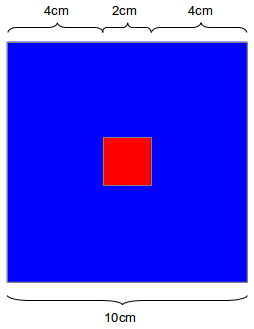
\includegraphics[width=3cm]{amr_zones}
  \caption{Regions of the AMR problem.}
  \label{amr_regions}
\end{figure}
The domain is a square of 10cm side (blue region) with in its center a smaller
square of 2cm side (red region). In the blue region, we have
$\Sigma_t=2cm^{-1}$ and $\Sigma_s=1cm^{-1}$. In the red region, we have
$\Sigma_t=1cm^{-1}$, $\Sigma_s=0.8cm^{-1}$, and a source of intensity $10
n/cm^{2}$. We use vacuum boundaries. The domain is initially discretize using
an uniform mesh of five by five cells. This mesh is then refined three
times. For each refinement, the cells with an estimated error of 70\% or more
of the largest estimated error are refined. \Cref{diffusion_amr} shows the
results.
\begin{figure}[H]
  \centering
  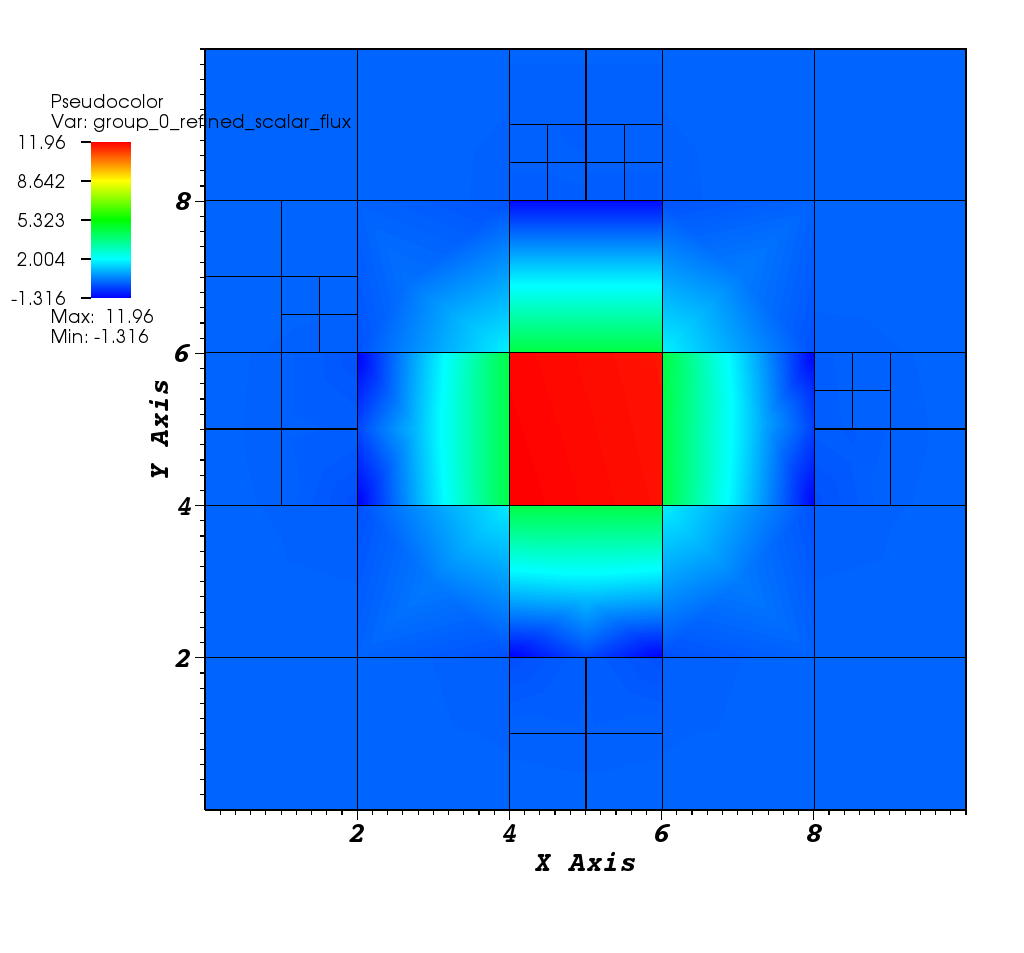
\includegraphics[width=5cm]{diffusion_amr}
  \caption{Solution of the AMR problem.}
  \label{diffusion_amr}
\end{figure}
\red{Je ne sais pas pourquoi ce ne sont pas pourquoi le raffinement est si
mauvais. Il y a surement un bug.}

\section{Conclusions}


% bibliography
\bibliographystyle{unsrt}
\bibliography{database}


\end{document}
